\documentclass{plt}
\usetheme{metropolis}           % Use metropolis theme

% Make | a mathrel symbol: improves alternation (a | b) spacing
\mathcode`\|="326A

\tikzset{double distance=1pt,>=latex}

\tikzset{
  parsetree/.style={
    level distance=2pc,
    sibling distance=1.8pc,
    every node/.style={fill=white},
    every path/.style={thick},
    baseline=(current bounding box.west)
  }
}

% For drawing arithmetic parse trees

\def\plus#1#2{node {\texttt{+}} child {#1} child {#2}}
\def\minus#1#2{node {\texttt{-}} child {#1} child {#2}}
\def\mult#1#2{node {\texttt{*}} child {#1} child {#2}}
\def\lit#1{node {#1}}

\tikzfading[name=fade down,
  top color=transparent!0,
  bottom color=transparent!100]

\tikzfading[name=fade up,
  bottom color=transparent!0,
  top color=transparent!100]

\newcommand{\pac}{\cdot}

\author{Review for the Midterm}
\institute{Columbia University}
\date{Spring 2019}
\titlegraphic{
\vspace{220pt}
{\tiny $^*$ Course website: \url{https://www.cs.columbia.edu/~rgu/courses/4115/spring2019}\vspace{-5pt}}\\
{\tiny $^{**}$ These slides are borrowed from Prof. Edwards.}
}


\begin{document}

\frame{\titlepage}

\frame{\footnotesize\parskip=0pt\tableofcontents}

\section{The Midterm}

\begin{frame}{The Midterm}

75 minutes

Closed book

One double-sided sheet of notes of your own devising

Anything discussed in class is fair game

Little, if any, programming

Details of OCaml/C/C++/Java syntax not required

\end{frame}

\section{Structure of a Compiler}

\begin{frame}[fragile]
  \frametitle{Compiling a Simple Program}

\begin{C}
int gcd(int a, int b)
{
  while (a != b) {
    if (a > b) a -= b;
    else b -= a;
  }
  return a;
}
\end{C}

\end{frame}

\newsavebox{\gcdbox}
\begin{lrbox}{\gcdbox}
\begin{minipage}{0.4\textwidth}
\begin{C}
int gcd(int a, int b)
{
  while (a != b) {
    if (a > b) a -= b;
    else b -= a;
  }
  return a;
}
\end{C}
\end{minipage}
\end{lrbox}

%%%%%%%%%%%%%%%%%%%%%%%%%%%%%%

\begin{frame}[fragile]
  \frametitle{What the Compiler Sees}

\usebox{\gcdbox}

\begin{verbatim}
i  n  t sp  g  c  d  (  i  n  t sp  a  , sp  i
n  t sp  b  ) nl  { nl sp sp  w  h  i  l  e sp
(  a sp  !  = sp  b  ) sp  { nl sp sp sp sp  i
f sp  (  a sp  > sp  b  ) sp  a sp  -  = sp  b
; nl sp sp sp sp  e  l  s  e sp  b sp  -  = sp
a  ; nl sp sp  } nl sp sp  r  e  t  u  r  n sp
a  ; nl  } nl
\end{verbatim}

Text file is a sequence of characters

\end{frame}

%%%%%%%%%%%%%%%%%%%%%%%%%%%%%%

\begin{frame}[fragile]
  \frametitle{Lexical Analysis Gives Tokens}

\usebox{\gcdbox}\hfill
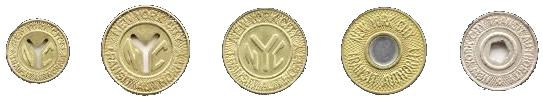
\includegraphics[width=0.45\textwidth]{subway-tokens.jpg}

\newbox\mystrutbox
\setbox\mystrutbox=\hbox{\vrule height7.5pt depth2.5pt width0pt}
\def\strut{\relax\ifmmode\copy\mystrutbox\else\unhcopy\mystrutbox\fi}

\def\frame #1 #2 #3 #4 #5 #6 #7 #8
{\framebox{\strut #1} 
\framebox{\strut #2} 
\framebox{\strut #3} 
\framebox{\strut #4}
\framebox{\strut #5} 
\framebox{\strut #6} 
\framebox{\strut #7} 
\framebox{\strut #8}
}

{\ttfamily
\frame int gcd ( int a , int b
\frame ) \{ while ( a != b )
\frame \{ if ( a $>$ b ) a
\frame -= b ; else b -= a ;
\framebox{\strut\}} \framebox{\strut return} \framebox{\strut a}
\framebox{\strut ;} \framebox{\strut \}}
}

A stream of tokens.  Whitespace, comments removed.

\end{frame}

\newcommand{\id}[1]{
  node [fill=white] {#1}
}

\newcommand{\theast}{
  \node {func} [level distance=2pc,
    level 1/.style={sibling distance=3.5pc},
    level 2/.style={sibling distance=4.5pc},
    level 3/.style={sibling distance=2.5pc},
    level 4/.style={sibling distance=2.5pc},
    level 5/.style={sibling distance=1.5pc},
  ]
  child {node {int}}
  child {node {gcd}}
  child {node {args}
    child {node {arg}
      child {node {int}}
      child {\id a}}
    child {node {arg}
      child {node {int}}
      child {\id b}}
  }
  child [missing]
  child [missing]
  child {node {seq}
    child {
      node {while}
      child {node {!=}
        child {\id a}
        child {\id b}
      }
      child [missing]
      child {
        node {if}
        child {
          node {>}
          child {\id a}
          child {\id b}}
        child {
          node {-=}
          child {\id a}
          child {\id b}}
        child {
          node {-=}
          child {\id b}
          child {\id a}}
      }
    }
    child {
      node {return}
      child {\id a}
    }
  }
  ;
}

\begin{frame}
  \frametitle{Parsing Gives an Abstract Syntax Tree}

\begin{tikzpicture}
  \theast
\end{tikzpicture}

\vspace{-3pc}
\usebox{\gcdbox}

\end{frame}

\renewcommand{\id}[1]{
  node [fill=white] (id) {#1}
  (id) .. controls +(-1,-2) and +(1,0) .. (#1.east)
}

\begin{frame}
  \frametitle{Semantic Analysis Resolves Symbols and Checks Types}

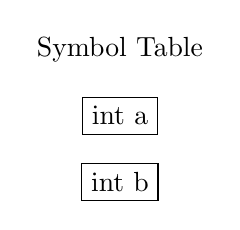
\begin{tikzpicture}
  \node at (-10pc, -8pc) {Symbol Table};
  \node [draw] at (-10pc,-10pc) (a) {int a};
  \node [draw] at (-10pc,-12pc) (b) {int b};
  \theast
\end{tikzpicture}

\end{frame}

%%%%%%%%%%%%%%%%%%%%%%%%%%%%%%

\begin{frame}[fragile]
  \frametitle{Translation into 3-Address Code}

\begin{assembly}
L0: sne   $1,  a, b
    seq   $0, $1, 0
    btrue $0, L1    # while (a != b)
    sl    $3,  b, a
    seq   $2, $3, 0
    btrue $2, L4    # if (a < b)
    sub   a,   a, b # a -= b
    jmp   L5
L4: sub   b,   b, a # b -= a
L5: jmp   L0
L1: ret    a
\end{assembly}

\usebox{\gcdbox}\hfill\parbox{14pc}{\raggedright
Idealized assembly language w/ infinite registers
}

% Generated from SUIF/MachSUIF:
%
% c2s gcd.c
% do_lower gcd.suif gcd.lsuif
% do_s2m gcd.lsuif gcd.suifvm
% do_print gcd.suifvm
%
% Heavily massaged to make it readable

\end{frame}

%%%%%%%%%%%%%%%%%%%%%%%%%%%%%%

\begin{frame}[fragile]
  \frametitle{Generation of 80386 Assembly}

\hfill 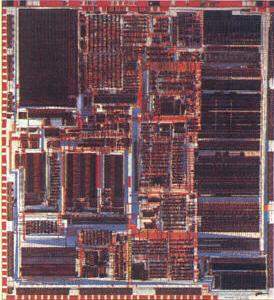
\includegraphics[width=5pc]{80386.jpg}

\begin{assembly}
gcd:  pushl %ebp          # Save BP
      movl  %esp,%ebp
      movl  8(%ebp),%eax  # Load a from stack
      movl  12(%ebp),%edx # Load b from stack
.L8:  cmpl  %edx,%eax
      je    .L3           # while (a != b)
      jle   .L5           # if (a < b)
      subl  %edx,%eax     # a -= b
      jmp   .L8
.L5:  subl  %eax,%edx     # b -= a
      jmp   .L8
.L3:  leave               # Restore SP, BP
      ret
\end{assembly}

\end{frame}

\section{Scanning}

\subsection{Languages and Regular Expressions}

\begin{frame}
  \frametitle{Describing Tokens}

\textbf{Alphabet}: A finite set of symbols

Examples: $\{$ 0, 1 $\}$, $\{$ A, B, C, \ldots, Z $\}$, ASCII, Unicode

\vfil

\textbf{String}: A finite sequence of symbols from an alphabet

Examples: $\epsilon$ (the empty string), Stephen, $\alpha\beta\gamma$

\vfil

\textbf{Language}: A set of strings over an alphabet

Examples: $\emptyset$ (the empty language), $\{$ 1, 11, 111, 1111
$\}$, all English words, strings that start with a letter followed by
any sequence of letters and digits

\end{frame}

\begin{frame}
  \frametitle{Operations on Languages}

Let $L = \{$ $\epsilon$, wo $\}$, $M = \{$ man, men $\}$

\vfil

\textbf{Concatenation}: Strings from one followed by the other

$LM = \{$ man, men, woman, women $\}$

\vfil

\textbf{Union}: All strings from each language

$L \cup M = \{ \epsilon, $ wo, man, men $\}$

\vfil

\textbf{Kleene Closure}: Zero or more concatenations

$M^* = \{ \epsilon \} \cup M \cup MM \cup MMM \cdots = \break
 \{ \epsilon, $ man, men, manman, manmen, menman, menmen,
manmanman, manmanmen, manmenman, \ldots $\}$

\end{frame}

\begin{frame}
  \frametitle{Regular Expressions over an Alphabet $\Sigma$}

A standard way to express languages for tokens.

\begin{enumerate}

\item $\epsilon$ is a regular expression that denotes $\{\epsilon\}$

\item If $a \in \Sigma$, $a$ is an RE that denotes $\{a\}$

\item If $r$ and $s$ denote languages $L(r)$ and $L(s)$,

\begin{itemize}

\item  $(r)|(s)$ denotes $L(r) \cup L(s)$
\item $(r)(s)$ denotes $\{ tu : t \in L(r), u \in L(s) \}$
\item $(r)^*$ denotes $\cup_{i=0}^{\infty} L^i$ ($L^0 =
  \{\epsilon\}$ and $L^i = L L^{i-1}$)
\end{itemize}

\end{enumerate}

\end{frame}

\subsection{NFAs}

\begin{frame}[fragile]
  \frametitle{Nondeterministic Finite Automata}

\begin{columns}
\begin{column}{0.4\textwidth}

``All strings containing an even number of 0's and 1's''

\vspace{2pc}

\begin{tikzpicture}
  \matrix [matrix of math nodes,
    nodes={circle,draw},
    column sep=2.5pc,
    row sep=2.5pc] {
    |[double] (A)| A & |(B)| B \\
    |(C)| C & |(D)| D \\
  };
  \begin{scope}[->, bend angle=15,bend left,inner sep=2pt]
    \draw (A) to node [above] {0} (B); 
    \draw (B) to node [below] {0} (A);
    \draw (B) to node [right] {1} (D); 
    \draw (D) to node [left]  {1} (B);
    \draw (D) to node [below] {0} (C); 
    \draw (C) to node [above] {0} (D);
    \draw (C) to node [left] {1} (A); 
    \draw (A) to node [right] {1} (C);
    \draw (A) ++ (-1.3pc,1pc) -- (A);
  \end{scope}
\end{tikzpicture}

\end{column}
\begin{column}{0.6\textwidth}

\begin{enumerate}\itemsep=0pt

\item Set of states $S:
\left\{
\begin{tikzpicture}[baseline=-4pt]
  \matrix [column sep=5pt,matrix of math nodes,nodes={circle,draw}] {
    |[double]| A & B & C & D \\ };
\end{tikzpicture}
\right\}$

\item Set of input symbols $\Sigma: \{ 0, 1 \}$

\item Transition function $\sigma : S \times \Sigma_{\epsilon} \rightarrow 2^S$

$\begin{array}{c|ccc}
\textbf{state} & \epsilon & 0 & 1 \\
\hline
A & \emptyset & \{B\} & \{C\} \\
B & \emptyset & \{A\} & \{D\} \\
C & \emptyset & \{D\} & \{A\} \\
D & \emptyset & \{C\} & \{B\} \\
\end{array}
$

\item Start state $s_0 :

\begin{tikzpicture}[baseline=-4pt]
  \node [draw,circle,double] {$A$};
\end{tikzpicture}
 $

\item Set of accepting states $F:
\left\{

\begin{tikzpicture}[baseline=-4pt]
  \node [draw,circle,double] {$A$};
\end{tikzpicture}
\right\}$

\end{enumerate}

\end{column}
\end{columns}

\end{frame}

\begin{frame}[fragile]
  \frametitle{The Language induced by an NFA}

An NFA accepts an input string $x$ iff there is a path from the start
state to an accepting state that ``spells out'' $x$.

\vspace{2pc}

\begin{center}
\begin{tikzpicture}
  \matrix [matrix of math nodes,
    nodes={circle,draw},
    column sep=2.5pc,
    row sep=2.5pc] {
    |[double] (A)| A & |(B)| B \\
    |(C)| C & |(D)| D \\
  };
  \begin{scope}[->, bend angle=15,bend left,inner sep=2pt]
    \draw (A) to node [above] {0} (B); 
    \draw (B) to node [below] {0} (A);
    \draw (B) to node [right] {1} (D); 
    \draw (D) to node [left]  {1} (B);
    \draw (D) to node [below] {0} (C); 
    \draw (C) to node [above] {0} (D);
    \draw (C) to node [left] {1} (A); 
    \draw (A) to node [right] {1} (C);
    \draw (A) ++ (-1.3pc,1pc) -- (A);
  \end{scope}
\end{tikzpicture}
\end{center}

Show that the string ``010010'' is accepted.

\begin{tikzpicture}
  \matrix (z) [matrix of math nodes,
    nodes={circle,draw},
    column sep=1.5pc] {
    |[double]| A & B & D & C & D & B & |[double]| A \\
  };
  \begin{scope}[->,every node/.style={above}]
    \draw (z-1-1) -- node {0} (z-1-2);
    \draw (z-1-2) -- node {1} (z-1-3);
    \draw (z-1-3) -- node {0} (z-1-4);
    \draw (z-1-4) -- node {0} (z-1-5);
    \draw (z-1-5) -- node {1} (z-1-6);
    \draw (z-1-6) -- node {0} (z-1-7);
  \end{scope}
\end{tikzpicture}

\end{frame}

\subsection{Translating REs into NFAs: Thompson's Construction}

\begin{frame}[fragile]
  \frametitle{Translating REs into NFAs}

\tikzset{every matrix/.style={matrix of math nodes,
                              nodes={circle,minimum size=1pc,draw}},
         initial text={},
         every state/.style={minimum size=1.5pc,fill=white},
         group/.style={ellipse,draw,fill=black!10,minimum height=2.7pc, inner sep=-5pt},
         node distance=0.5pc and 2pc}

\begin{tabular}{ccc}
$a$ &
\begin{tikzpicture}[baseline=-4pt]
  \node[state,initial]              (A) {};
  \node[state,accepting,right=of A] (B) {};
  \path [->] (A) edge node [above] {$a$} (B);
\end{tikzpicture}
&
Symbol
\\[1pc]
$r_1 r_2$ &
\begin{tikzpicture}[baseline=-4pt]
  \node [state,initial]              (A) {};
  \node [state,right=of A]           (B) {};
  \node [state,accepting,right=of B] (C) {};
  \begin{pgfonlayer}{background}
    \node [group,fit=(A) (B)] {$r_1$};
    \node [group,fit=(B) (C)] {$r_2$};
  \end{pgfonlayer}
  \node [group,fill=none,fit=(A) (B)] {$r_1$};
\end{tikzpicture}
&
Sequence
\\[2pc]
$r_1 | r_2$ &
\begin{tikzpicture}[baseline=-4pt]
  \node [state,initial]              (A) {};
  \node [state,above right=of A]     (B) {};
  \node [state,right=of B]           (C) {};
  \node [state,accepting,below right=of C] (D) {};
  \node [state,below right=of A]     (E) {};
  \node [state,right=of E]     (F) {};
  \begin{pgfonlayer}{background}
    \node [group,fit=(B) (C)] {$r_1$};
    \node [group,fit=(E) (F)] {$r_2$};
  \end{pgfonlayer}
  \path [->] (A) edge node [above left] {$\epsilon$} (B)
             (A) edge node [below left] {$\epsilon$} (E)
             (C) edge node [above right] {$\epsilon$} (D)
             (F) edge node [below right] {$\epsilon$} (D);
\end{tikzpicture}
&
Choice
\\[3pc]
$(r)^*$ &
\begin{tikzpicture}[baseline=-4pt]
  \node [state,initial]              (A) {};
  \node [state,right=of A]           (B) {};
  \node [state,right=of B]           (C) {};
  \node [state,accepting,right=of C] (D) {};
  \begin{pgfonlayer}{background}
    \node [group,fit=(B) (C)] {$r$};
  \end{pgfonlayer}
  \path [->] (A) edge              node [above] {$\epsilon$} (B)
             (C) edge              node [above] {$\epsilon$} (D)
             (C) edge [bend right=80] node [above] {$\epsilon$} (B)
             (A) edge [bend right=40] node [below] {$\epsilon$} (D);
\end{tikzpicture}
&
Kleene Closure
 \\
\end{tabular}

\end{frame}

\def\filled#1{\ifx#11red\else white\fi}

\def\aabb#1#2#3#4#5#6#7#8#9{
  \begin{tikzpicture}[node distance=0.7pc and 1pc,                      
                      every state/.style={inner sep=1pt,
                        fill=white,
                        minimum size=14pt},
                        initial text={}]
    \node [state,fill=\filled#1,initial] (0) {0};
    \node [state,fill=\filled#2,right=of 0] (1) {1};
    \node [state,fill=\filled#3,above right=of 1] (2) {2};
    \node [state,fill=\filled#4,right=of 2] (3) {3};
    \node [state,fill=\filled#5,below right=of 1] (4) {4};
    \node [state,fill=\filled#6,right=of 4] (5) {5};
    \node [state,fill=\filled#7,below right=of 3] (6) {6};
    \node [state,fill=\filled#8,right=of 6] (7) {7};
    \node [state,fill=\filled#9,right=of 7] (8) {8};
\aabbtwo
}

\def\aabbtwo#1#2{
    \node [state,fill=\filled#1,right=of 8] (9) {9};
    \node [state,fill=\filled#2,accepting,right=of 9] (10) {10};
    \path [->] (0) edge node [above] {$\epsilon$} (1)
               (1) edge node [above left] {$\epsilon$} (2)
               (2) edge node [above] {$a$} (3)
               (1) edge node [below left] {$\epsilon$} (4)
               (4) edge node [below] {$b$} (5)            
               (3) edge node [above right] {$\epsilon$} (6)
               (5) edge node [below right] {$\epsilon$} (6)
               (6) edge node [above] {$\epsilon$} (7)
               (7) edge node [above] {$a$} (8)
               (8) edge node [above] {$b$} (9)
               (9) edge node [above] {$b$} (10)
               (6) edge [bend right=90,looseness=1.5] node [above] {$\epsilon$} (1)
               (0) edge [bend right=70] node [below] {$\epsilon$} (7)
            ;
  \end{tikzpicture}
}

\begin{frame}[fragile]
  \frametitle{Translating REs into NFAs}

Example: Translate $(a|b)^*abb$ into an NFA. Answer:

\aabb00000000000

Show that the string ``$aabb$'' is accepted. Answer:

\begin{tikzpicture}[node distance=1pc,every state/.style={inner sep=1pt,minimum size=14pt},
    initial text={}]
  \node [state,initial] (0) {0};
  \node [state,right=of 0] (1) {1};
  \node [state,right=of 1] (2) {2};
  \node [state,right=of 2] (3) {3};
  \node [state,right=of 3] (6) {6};
  \node [state,right=of 6] (7) {7};
  \node [state,right=of 7] (8) {8};
  \node [state,right=of 8] (9) {9};
  \node [state,right=of 9,accepting] (10) {10};
  \path [->] (0) edge node [above] {$\epsilon$} (1)
             (1) edge node [above] {$\epsilon$} (2)
             (2) edge node [above] {$a$} (3)
             (3) edge node [above] {$\epsilon$} (6)
             (6) edge node [above] {$\epsilon$} (7)
             (7) edge node [above] {$a$} (8)
             (8) edge node [above] {$b$} (9)
             (9) edge node [above] {$b$} (10)
  ;
\end{tikzpicture}


\end{frame}


\begin{frame}
  \frametitle{Deterministic Finite Automata}

Restricted form of NFAs:

\begin{itemize}
\item No state has a transition on $\epsilon$
\item For each state $s$ and symbol $a$, there is at most one edge
  labeled $a$ leaving $s$.
\end{itemize}

Differs subtly from the definition used in COMS W3261 (Sipser,
\emph{Introduction to the Theory of Computation})

Very easy to check acceptance: simulate by maintaining current state.
Accept if you end up on an accepting state. Reject if you end on a
non-accepting state or if there is no transition from the current
state for the next symbol.

\end{frame}

\begin{frame}[fragile]
  \frametitle{Deterministic Finite Automata}

\begin{ocamllex}
{
   type token = ELSE | ELSEIF
}

rule token =
  parse "else"   { ELSE }
      | "elseif" { ELSEIF }
\end{ocamllex}

\begin{tikzpicture}[node distance=1.5pc,
    every state/.style={inner sep=1pt,minimum size=14pt},
    initial text={}]
  \node [state,initial] (0) {};
  \node [state,right=of 0] (1) {};
  \node [state,right=of 1] (2) {};
  \node [state,right=of 2] (3) {};
  \node [state,right=of 3,accepting] (4) {};
  \node [state,right=of 4] (5) {};
  \node [state,right=of 5,accepting] (6) {};
  \path [->] (0) edge node [above] {e} (1)
             (1) edge node [above] {l} (2)
             (2) edge node [above] {s} (3)
             (3) edge node [above] {e} (4)
             (4) edge node [above] {i} (5)
             (5) edge node [above] {f} (6);
\end{tikzpicture}

\end{frame}


\begin{frame}[fragile]
  \frametitle{Deterministic Finite Automata}

\begin{ocamllex}
{ type token = IF | ID of string | NUM of string }

rule token =
  parse "if"                                { IF }
      | ['a'-'z'] ['a'-'z' '0'-'9']* as lit { ID(lit) }
      | ['0'-'9']+                   as num { NUM(num) }
\end{ocamllex}

\begin{tikzpicture}
[node distance=3pc and 5pc,
    every state/.style={inner sep=1pt,minimum size=30pt},
    initial text={}]
  \node [state,initial] (start) {};
  \node [state,below right=of start,accepting] (num) {NUM};
  \node [state,above right=of start,accepting] (id1) {ID};
  \node [state,right=of id1,accepting] (if) {IF};
  \node [state,below=of if,accepting] (id2) {ID};
  \path [->] (start) edge node [below left] {0--9} (num)
             (start) edge node [above] {i} (id1)
             (start) edge node [above] {a--hj--z} (id2)
             (id1) edge node [above] {f} (if)
             (if) edge node [right] {a--z0--9} (id2)
             (id1) edge node [above,sloped] {a--eg--z0--9} (id2)
             (num) edge [loop right] node [right] {0--9} ()
             (id2) edge [loop right] node [right] {a--z0--9} ();
\end{tikzpicture}

\end{frame}

\subsection{Building a DFA from an NFA: Subset Construction}

\begin{frame}
  \frametitle{Building a DFA from an NFA}

Subset construction algorithm

Simulate the NFA for all possible inputs and track the states that
appear.

Each unique state during simulation becomes a state in the DFA.

\end{frame}

\def\aabb#1#2#3#4#5#6#7#8#9{
\begin{scope}[node distance=3pt and 2pt,
                      every state/.style={inner sep=1pt,
                        fill=white,
                        minimum size=5pt}]
    \node [state,fill=\filled#2] at ($(#1)+(left:1)$) (0) {};
    \node [state,fill=\filled#3,right=of 0] (1) {};
    \node [state,fill=\filled#4,above right=of 1] (2) {};
    \node [state,fill=\filled#5,right=of 2] (3) {};
    \node [state,fill=\filled#6,below right=of 1] (4) {};
    \node [state,fill=\filled#7,right=of 4] (5) {};
    \node [state,fill=\filled#8,below right=of 3] (6) {};
    \node [state,fill=\filled#9,right=of 6] (7) {};
\aabbtwo
}

\def\aabbtwo#1#2#3{
    \node [state,fill=\filled#1,right=of 7] (8) {};
    \node [state,fill=\filled#2,right=of 8] (9) {};
    \node [state,fill=\filled#3,accepting,right=of 9] (10) {};
    \path (0) edge node [above] {} (1)
          (1) edge node [above left] {} (2)
          (2) edge node [above] {} (3)
          (1) edge node [below left] {} (4)
          (4) edge node [below] {} (5)            
          (3) edge node [above right] {} (6)
          (5) edge node [below right] {} (6)
          (6) edge node [above] {} (7)
          (7) edge node [above] {} (8)
          (8) edge node [above] {} (9)
          (9) edge node [above] {} (10)
          (6) edge [bend right=90,looseness=2.5] node [above] {} (1)
          (0) edge [bend right=80,looseness=1.5] node [below] {} (7)
            ;
\end{scope}
}

%                  01234567890
\def\sa#1{\aabb{#1}11101001000}
\def\sb#1{\aabb{#1}01111011100}
\def\sc#1{\aabb{#1}01101111000}
\def\sd#1{\aabb{#1}01101111010}
\def\se#1{\aabb{#1}01101111001}

% sa -a-> sb -a-> sb -b-> sd -b-> se
% sa -b-> sc -b-> sc -a-> sb
% sd -a-> sb
% se -a-> sb
% se -b-> sc

\begin{frame}[t]
  \frametitle{Subset construction for $(a|b)^*abb$}
  \begin{tikzpicture}[nfastate/.style={state,inner sep=25pt},
    initial text={}]
    \node [initial,nfastate] (a) {};
    \sa{a}
    \pause
    \node [nfastate,right=of a] (b) {}; % \sb \\ };
    \sb{b}
    \node [nfastate,below=of a] (c) {}; % \sc \\ };
    \sc{c}
    \path [->] (a) edge node [above] {a} (b)
               (a) edge node [left] {b} (c);
    \pause
    \node [nfastate,right=of b] (d) {};% \sd \\ };
    \sd{d}
    \path [->,every loop/.style={looseness=3}]
               (b) edge [loop above] node [above] {a} ()
               (b) edge [bend left=20] node [above] {b} (d)
               (c) edge [loop left] node [left] {b} ()
               (c) edge node [below right] {a} (b);
    \pause
    \node [nfastate,accepting,below=of d] (e) {};% \se \\ };
    \se{e}
    \path [->]
          (d) edge [bend left=20] node[below] {a} (b)
          (d) edge node [right] {b} (e);
    \pause
    \path [->]
          (e) edge node [below left] {a} (b)
          (e) edge node [below] {b} (c);
  \end{tikzpicture}
\end{frame}

\begin{frame}
  \frametitle{Result of subset construction for $(a|b)^*abb$}
\begin{center}
  \begin{tikzpicture}[node distance=4pc,initial text={}]
    \node [initial,state] (a) {};
    \node [state,right=of a] (b) {};
    \node [state,below=of a] (c) {};
    \path [->] (a) edge node [above] {a} (b)
               (a) edge node [left] {b} (c);
    \node [state,right=of b] (d) {};
    \path [->,every loop/.style={looseness=3}]
               (b) edge [loop above] node [above] {a} ()
               (b) edge [bend left=20] node [above] {b} (d)
               (c) edge [loop left] node [left] {b} ()
               (c) edge node [below right] {a} (b);
    \node [state,accepting,below=of d] (e) {};
    \path [->]
          (d) edge [bend left=20] node[below] {a} (b)
          (d) edge node [right] {b} (e);
    \path [->]
          (e) edge node [below left] {a} (b)
          (e) edge node [below] {b} (c);
  \end{tikzpicture}

  \emph{Is this minimal?}

  (Subset construction does not involve minimization)
\end{center}
\end{frame}

\section{Parsing}

\subsection{Resolving Ambiguity}

\begin{frame}
  \frametitle{Ambiguous Arithmetic}

Ambiguity can be a problem in expressions.  Consider parsing

\begin{center}
\texttt{3 - 4 * 2 + 5}
\end{center}

with the grammar

\[e \rightarrow  e + e | e - e | e * e | e \mathop{/} e | N\]

\ttfamily

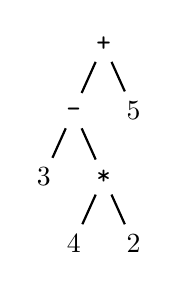
\begin{tikzpicture}[parsetree]
  \path
    \plus{\minus{\lit3}
                {\mult{\lit4}{\lit2}}}
         {\lit5}
    ;
\end{tikzpicture}
\hfil
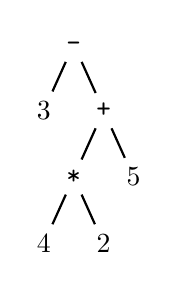
\begin{tikzpicture}[parsetree]
  \path
    \minus{\lit3}
          {\plus{\mult{\lit4}{\lit2}}
                {\lit5}}
    ;
\end{tikzpicture}
\hfil
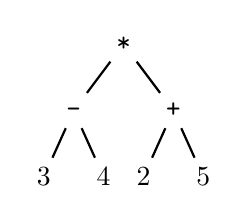
\begin{tikzpicture}[parsetree,
                 level 1/.style={sibling distance=3pc},
                 level 2/.style={sibling distance=1.8pc}]
  \path \mult{\minus{\lit3}{\lit4}}
              {\plus{\lit2}{\lit5}}
    ;
\end{tikzpicture}
\hfil
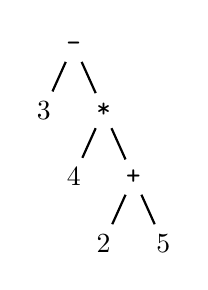
\begin{tikzpicture}[parsetree]
  \path \minus{\lit3}
              {\mult{\lit4}
                     {\plus{\lit2}{\lit5}}};
\end{tikzpicture}
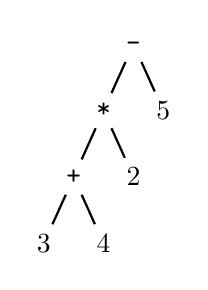
\begin{tikzpicture}[parsetree]
  \path \minus{\mult{\plus{\lit3}{\lit4}}{\lit2}}{\lit5};
\end{tikzpicture}

\end{frame}

\begin{frame}
  \frametitle{Operator Precedence}

Defines how ``sticky'' an operator is.

\begin{center}\ttfamily
1 * 2 + 3 * 4
\end{center}

\begin{minipage}{0.65\textwidth}
\texttt{*} at higher precedence than \texttt{+}:

\medskip

\texttt{(1 * 2) + (3 * 4)}
\end{minipage}
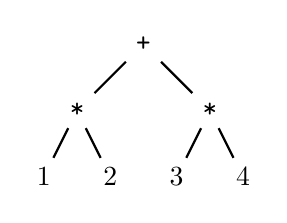
\begin{tikzpicture}[parsetree,
    level 1/.style={sibling distance=4pc},
    level 2/.style={sibling distance=2pc}]
  \path
  \plus{\mult{\lit1}{\lit2}}
       {\mult{\lit3}{\lit4}};
\end{tikzpicture}

\begin{minipage}{0.65\textwidth}
\texttt{+} at higher precedence than \texttt{*}:

\medskip

\texttt{1 * (2 + 3) * 4}
\end{minipage}
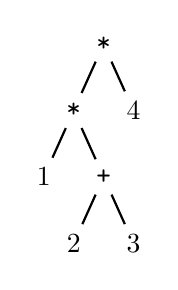
\begin{tikzpicture}[parsetree]
  \path
  \mult{\mult{\lit1}
               {\plus{\lit2}{\lit3}}}
        {\lit4};
\end{tikzpicture}
\end{frame}

\begin{frame}
  \frametitle{Associativity}

Whether to evaluate left-to-right or right-to-left

Most operators are left-associative

\begin{center}
\texttt{1 - 2 - 3 - 4}

\vspace{2pc}

\begin{tabular}{c@{\hspace{5pc}}c}
  \ttfamily
  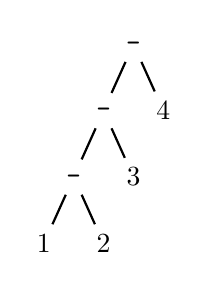
\begin{tikzpicture}[parsetree]
    \path \minus{\minus{\minus{\lit1}{\lit2}}{\lit3}}{\lit4};
  \end{tikzpicture}
&
  \ttfamily
  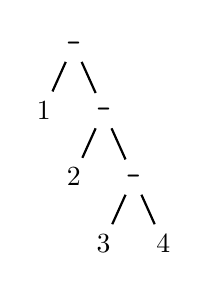
\begin{tikzpicture}[parsetree]
    \path \minus{\lit1}{\minus{\lit2}{\minus{\lit3}{\lit4}}};
  \end{tikzpicture}
\\
\\
$((1 - 2) - 3) - 4$ & $1 - (2 - (3 - 4))$ \\
\\
left associative & right associative
\end{tabular}

\end{center}

\end{frame}

\begin{frame}[fragile]
  \frametitle{Fixing Ambiguous Grammars}

A grammar specification:

\begin{ocamlyacc}
expr :
    expr PLUS expr  
  | expr MINUS expr 
  | expr TIMES expr 
  | expr DIVIDE expr
  | NUMBER          
\end{ocamlyacc}

Ambiguous: no precedence or associativity.

Ocamlyacc's complaint: ``16 shift/reduce conflicts.''

\end{frame}

\begin{frame}[fragile]
  \frametitle{Assigning Precedence Levels}

Split into multiple rules, one per level

\begin{ocamlyacc}
expr : expr PLUS expr  
     | expr MINUS expr 
     | term            

term : term TIMES term 
     | term DIVIDE term
     | atom            

atom  : NUMBER         
\end{ocamlyacc}

Still ambiguous: associativity not defined

Ocamlyacc's complaint: ``8 shift/reduce conflicts.''

\end{frame}

\begin{frame}[fragile]
  \frametitle{Assigning Associativity}

Make one side the next level of precedence

\begin{ocamlyacc}
expr : expr PLUS term  
     | expr MINUS term 
     | term            

term : term TIMES atom 
     | term DIVIDE atom
     | atom            

atom  : NUMBER         
\end{ocamlyacc}

This is left-associative.

No shift/reduce conflicts.

\end{frame}

\renewcommand{\id}{\textbf{Id}}

\newcommand{\handle}[3]{
  \begin{tikzpicture}
    \node [inner sep=1pt] (n1) {$#1$};
    \node [inner sep=1pt,anchor=base west] (n2) at (n1.base east) {$#2$};
    \node [inner sep=1pt,anchor=base west] (n1) at (n2.base east) {$#3$};
    \draw ($(n2.south west) + (-1pt,-1pt)$) --
          ($(n2.south east) + (1pt,-1pt)$);

\if 0
    \begin{pgfonlayer}{background}
      \draw [red!70,line width=2pt,rounded corners]
      ($(n2.north east) + (1pt,1pt)$) --
      ($(n2.north west) + (-1pt,1pt)$) --
      ($(n2.south west) + (-1pt,-1pt)$) --
      ($(n2.south east) + (1pt,-1pt)$) -- cycle
      ;
    \end{pgfonlayer}
\fi
  \end{tikzpicture}
}

\newcommand{\expand}[3]{
  \draw ($(#2.south west) + (1pt,0pt)$) -- 
        ($(#3.south east) + (-1pt,0pt)$);
\if 0
    \fill [even odd rule,red,path fading=fade up]
    (#1.north west)  [rounded corners] -- (#1.south west) --
    (#2.north west) -- (#2.south west) -- (#3.south east) --
    (#3.north east) -- (#1.south east) -- (#1.north east)
    -- cycle
    ($(#3.north east) + (-1pt,-1pt)$) --
    ($(#2.north west) + (1pt,-1pt)$) --
    ($(#2.south west) + (1pt,1pt)$) --
    ($(#3.south east) + (-1pt,1pt)$) -- cycle
    ;
\fi
}

\newcommand{\expandup}[3]{
  \draw ($(#2.south west) + (1pt,0pt)$) -- 
        ($(#3.south east) + (-1pt,0pt)$);
\if 0
    \fill [even odd rule,red,path fading=fade down]
    (#1.south west)  [rounded corners] -- (#1.north west) --
    (#2.south west) -- (#2.north west) -- (#3.north east) --
    (#3.south east) -- (#1.north east) -- (#1.south east)
    -- cycle
    ($(#3.south east) + (-1pt,1pt)$) --
    ($(#2.south west) + (1pt,1pt)$) --
    ($(#2.north west) + (1pt,-1pt)$) --
    ($(#3.north east) + (-1pt,-1pt)$) -- cycle
    ;
\fi
}

\newcommand{\grammarone}{
\renewcommand{\arraystretch}{1}
$\begin{array}[t]{@{}l@{\,}r@{\,}c@{\,}l@{}}
1: & e & \rightarrow & t + e \\
2: & e & \rightarrow & t \\
3: & t & \rightarrow & \id\ * t \\
4: & t & \rightarrow & \id
\end{array}$
}


\newenvironment{parsermoves}{
\begingroup
\small
\renewcommand{\arraystretch}{0.8}
\newcommand{\s}[2]{%
  \begin{pspicture}(10pt,10pt)
    \psframe(0,-5pt)(8pt,5pt)
    \rput(4pt,2pt){\tiny##1}
    \rput(4pt,-2pt){\tiny##2}
  \end{pspicture}}
\begin{tabular}[t]{l@{}rl}
\multicolumn{1}{c}{\hbox to 5em{\hss stack\hss}} & \multicolumn{1}{c}{input}
& \multicolumn{1}{c}{action} \\
}{
\end{tabular}
\endgroup
}


\newsavebox{\rightmostDerivation}
\begin{lrbox}{\rightmostDerivation}
  \begin{tikzpicture}[every node/.style={anchor=base,inner sep=2pt},
                      node distance=0pt]
  \node (t1) {$e$};
  \node [below=of t1,matrix of math nodes,inner sep=0pt] (t2) {
    t & + & |(t3)| e \\ };
  \node [below=of t2,matrix of math nodes] (t4) {
    t & + & |(t5)| t \\ };
  \node [below=of t4,matrix of math nodes] (t6) {
    |(t8)| t & + & |(t7)| \id \\ };
  \node [below=of t6,matrix of math nodes] (t9) {
    |(t10)| \id & * & |(t10a)| t & + & \id \\ };
  \node [below=of t9,matrix of math nodes] (t11) {
    \id & * & |(t12)| \id & + & \id \\ };
  \begin{pgfonlayer}{background}
    \expand{t1}{t2}{t2}
    \expand{t3}{t5}{t5}
    \expand{t5}{t7}{t7}
    \expand{t8}{t10}{t10a}
    \expand{t10a}{t12}{t12}
  \end{pgfonlayer}
      \end{tikzpicture}
\end{lrbox}

\newsavebox{\automataPatterns}
\begin{lrbox}{\automataPatterns}
\footnotesize\renewcommand{\arraystretch}{1}
\begin{tabular}[t]{l}
\handle{\id * \id * \cdots * }{\id * t}{\cdots} \\
\handle{\id * \id * \cdots * }{\id}{\cdots} \\
\handle{t + t + \cdots + }{t+e}{} \\
\handle{t + t + \cdots + t + }{\id}{} \\
\handle{t + t + \cdots + t + \id * \id * \cdots * }{\id * t}{} \\
\handle{t + t + \cdots + }{t}{} \\
\end{tabular}
\end{lrbox}

\section{Rightmost and Reverse-Rightmost Derivations}

\begin{frame}[t,fragile]
  \frametitle{Rightmost Derivation of $\id * \id + \id$}

\begin{columns}
  \begin{column}{0.3\textwidth}
    \grammarone
  \end{column}
  \begin{column}{0.7\textwidth}

\begin{center}
\begin{tikzpicture}[every node/.style={anchor=base,inner sep=2pt},
  node distance=0.3pc]
  \node (t1) {$e$};
  \node [below=of t1,matrix of math nodes,inner sep=0pt] (t2) {
    t & + & |(t3)| e \\ };
  \node [below=of t2,matrix of math nodes] (t4) {
    t & + & |(t5)| t \\ };
  \node [below=of t4,matrix of math nodes] (t6) {
    |(t8)| t & + & |(t7)| \id \\ };
  \node [below=of t6,matrix of math nodes] (t9) {
    |(t10)| \id & * & |(t10a)| t & + & \id \\ };
  \node [below=of t9,matrix of math nodes] (t11) {
    \id & * & |(t12)| \id & + & \id \\ };
  \begin{pgfonlayer}{background}
    \expand{t1}{t2}{t2}
    \expand{t3}{t5}{t5}
    \expand{t5}{t7}{t7}
    \expand{t8}{t10}{t10a}
    \expand{t10a}{t12}{t12}
  \end{pgfonlayer}
\end{tikzpicture}
\end{center}
  \end{column}
\end{columns}

\begin{center}

At each step, expand the \emph{rightmost} nonterminal.

\begin{tikzpicture}[node distance=0.5pc]
  \node (nt) {nonterminal};
  \node [below=of nt] (h)
        {``handle'': The right side of a production};
  \begin{pgfonlayer}{background}
    \expand{nt}{h}{h}
  \end{pgfonlayer}
\end{tikzpicture}

Fun and interesting fact: there is exactly one rightmost expansion if
the grammar is unambigious.

\end{center}

\end{frame}

\begin{frame}[t,fragile]
  \frametitle{Rightmost Derivation: What to Expand}

\begin{columns}
  \begin{column}{0.3\textwidth}
    \grammarone
  \end{column}
  \begin{column}{0.7\textwidth}
    \begin{center}
      \usebox{\rightmostDerivation}
    \end{center}
  \end{column}
\end{columns}

\begin{center}
  \begin{tikzpicture}[every node/.style={inner sep=2pt}]
  \node [anchor=east] (t1) {$e$};
  \node [anchor=east,matrix of math nodes,inner sep=0pt] at (0,-1.5pc) (t2) {
    t & + & |(t3)| e \\ };
  \node [anchor=east,matrix of math nodes] at (0,-3pc) (t4) {
    t & + & |(t5)| t \\ };
  \node [anchor=t8.east,matrix of math nodes] at (0,-4.5pc) (t6) {
    |(t8)| t & + & |(t7)| \id \\ };
  \node [anchor=t10a.east,matrix of math nodes] at (0,-6pc) (t9) {
    |(t10)| \id & * & |(t10a)| t & + & \id \\ };
  \node [anchor=west,matrix of math nodes] at (0,-7.5pc) (t11) {
    \id & * & |(t12)| \id & + & \id \\ };
  \begin{pgfonlayer}{background}
    \fill [black!10] (t1.north east) [rounded corners] rectangle +(-6pc,-9pc)
          node [black,below right] {Expand here $\uparrow$};
    \fill [black!10] ($(t1.north east) + (2pt,0)$)
          [rounded corners] rectangle +(6pc,-9pc)
          node [black,below] {Terminals only};
    \expand{t1}{t2}{t2}
    \expand{t3}{t5}{t5}
    \expand{t5}{t7}{t7}
    \expand{t8}{t10}{t10a}
    \expand{t10a}{t12}{t12}
  \end{pgfonlayer}
  \end{tikzpicture}
\end{center}

\end{frame}

\begin{frame}[t,fragile]
  \frametitle{Reverse Rightmost Derivation}

\begin{columns}
  \begin{column}{0.3\textwidth}
    \grammarone
  \end{column}
  \begin{column}{0.7\textwidth}
    \begin{center}
      \usebox{\rightmostDerivation}
    \end{center}
  \end{column}
\end{columns}

\begin{center}
  \begin{tikzpicture}[every node/.style={inner sep=1pt}]
  \node [anchor=west,matrix of math nodes] at (0,0) (t11) {
    \id & * & |(t12)| \id & + & \id \\ };
  \node (h10) at (9.8pc,0pc) {\id};
  \node (h9) at (9.8pc,-1.5pc) {$t$};
  \draw (h10) to (h9);
  \node [anchor=t10a.east,matrix of math nodes] at (0,-1.5pc) (t9) {
    |(t10)| \id & * & |(t10a)| t & + & \id \\ };
  \node (h8) at (8.8pc,-1.5pc) {$*$};
  \node (h7) at (7.8pc,-1.5pc) {\id};
  \node (h6) at (8.8pc,-3pc) {$t$};
  \draw (h6) to (h7)
        (h6) to (h8)
        (h6) to (h9);
  \node [anchor=t8.east,matrix of math nodes] at (0,-3pc) (t6) {
    |(t8)| t & + & |(t7)| \id \\ };
  \node (h5) at (10.6pc,-3pc) {\id};
  \node (h4) at (10.6pc,-4.5pc) {$t$};
  \draw (h4) to (h5);
  \node [anchor=east,matrix of math nodes] at (0,-4.5pc) (t4) {
    t & + & |(t5)| t \\ };
  \node (h3) at (10.6pc,-6pc) {$e$};
  \draw (h3) to (h4);
  \node [anchor=east,matrix of math nodes] at (0,-6pc) (t2) {
    t & + & |(t3)| e \\ };
  \node (h1) at (8.8pc,-7.5pc) {$e$};
  \node (h2) at (9.6pc,-6pc) {$+$};
  \draw (h1) to (h2)
        (h1) to (h3)
        (h1) to (h6);
  \node [anchor=east] (t1) at (0,-7.5pc) {$e$};
  \begin{pgfonlayer}{background}
    \fill [black!10] (t11.north west) [rounded corners] rectangle +(-6pc,-9pc)
          node [black,below right] {viable prefixes};
    \fill [black!10] ($(t11.north west) + (2pt,0)$)
          [rounded corners] rectangle +(6pc,-9pc)
          node [black,below left] {terminals};
    \expandup{t1}{t2}{t2}
    \expandup{t3}{t5}{t5}
    \expandup{t5}{t7}{t7}
    \expandup{t8}{t10}{t10a}
    \expandup{t10a}{t12}{t12}
  \end{pgfonlayer}
  \end{tikzpicture}
\end{center}

\end{frame}

\begin{frame}[fragile,t]
  \frametitle{Shift/Reduce Parsing Using an Oracle}

\begin{columns}
  \begin{column}{0.3\textwidth}
    \grammarone
  \end{column}
  \begin{column}{0.7\textwidth}
    \begin{center}
      \usebox{\rightmostDerivation}
    \end{center}
  \end{column}
\end{columns}

\begin{center}
  \begin{tikzpicture}[every node/.style={inner sep=1pt}]
  \node [anchor=west,matrix of math nodes] at (0,0) (t0) {
    \id & * & \id & + & \id \\ };
  \node [anchor=west] at (6.5pc,0pc) {shift};
%  \pause
  \node [anchor=t1.east,matrix of math nodes] at (0,-1pc) {
    |(t1)| \id & * & \id & + & \id \\ };
  \node [anchor=west] at (6.5pc,-1pc) {shift};
%  \pause
  \node [anchor=t2.east,matrix of math nodes] at (0,-2pc) {
    \id & |(t2)| * & \id & + & \id \\ };
  \node [anchor=west] at (6.5pc,-2pc) {shift};
%  \pause
  \node [anchor=t3.east,matrix of math nodes] at (0,-3pc) {
    \id & * &  |(t3)| \id & + & \id \\ };
  \node [anchor=west] at (6.5pc,-3pc) {reduce 4};
%  \pause
  \node [anchor=t4.east,matrix of math nodes] at (0,-4pc) {
    |(t5)| \id & * &  |(t4)| t & + & \id \\ };
  \node [anchor=west] at (6.5pc,-4pc) {reduce 3};
%  \pause
  \node [anchor=t6.east,matrix of math nodes] at (0,-5pc) {
    |(t6)| t & + & \id \\ };
  \node [anchor=west] at (6.5pc,-5pc) {shift};
%  \pause
  \node [anchor=t7.east,matrix of math nodes] at (0,-6pc) {
    t & |(t7)| + & \id \\ };
  \node [anchor=west] at (6.5pc,-6pc) {shift};
%  \pause
  \node [anchor=t8.east,matrix of math nodes] at (0,-7pc) {
    t & + & |(t8)| \id \\ };
  \node [anchor=west] at (6.5pc,-7pc) {reduce 4};
%  \pause
  \node [anchor=t9.east,matrix of math nodes] at (0,-8pc) {
    t & + & |(t9)| t \\ };
  \node [anchor=west] at (6.5pc,-8pc) {reduce 2};
%  \pause
  \node [anchor=t10.east,matrix of math nodes] at (0,-9pc) {
    |(t11)| t & + & |(t10)| e \\ };
  \node [anchor=west] at (6.5pc,-9pc) {reduce 1};
%  \pause
  \node [anchor=east] at (0,-10pc) (t12) {$e$};
  \node [anchor=west] at (6.5pc,-10pc) {accept};
  \begin{pgfonlayer}{background}
    \fill [black!10] (t0.north west) [rounded corners] rectangle +(-6pc,-11pc)
          node [black,below right] {stack};
    \fill [black!10] ($(t0.north west) + (2pt,0)$)
          [rounded corners] rectangle +(6pc,-11pc)
          node [black,below left] {input};
    \expandup{t4}{t3}{t3}
    \expandup{t6}{t5}{t4}
    \expandup{t9}{t8}{t8}
    \expandup{t10}{t9}{t9}
    \expandup{t12}{t11}{t10}
  \end{pgfonlayer}
  \end{tikzpicture}
\end{center}

\end{frame}

\begin{frame}
  \frametitle{Handle Hunting}

\textbf{Right Sentential Form:} any step in a rightmost derivation

\textbf{Handle:} in a sentential form, a RHS of a rule that, when
rewritten, yields the previous step in a rightmost derivation.

The big question in shift/reduce parsing:

\begin{center}
When is there a handle on the top of the stack?
\end{center}

Enumerate all the right-sentential forms and pattern-match against
them? \emph{Usually infinite in number, but let's try anyway.}

\end{frame}

\begin{frame}
  \frametitle{The Handle-Identifying Automaton}

Magical result, due to Knuth:  \emph{An automaton suffices to locate a handle
  in a right-sentential form.}

\begin{columns}
  \begin{column}{0.6\textwidth}
    \usebox{\automataPatterns}
  \end{column}
  \begin{column}{0.4\textwidth}
\begin{tikzpicture}[node distance=1.2pc and 2pc,initial text={},
    every state/.style={minimum size=28pt}]
  \node [state,initial] (S0) {};
  \node [state,below=of S0,accepting] (S1) {$\id$};
  \node [state,right=of S0,accepting] (S2) {$t$};
  \node [state,below=of S1] (S3) {};
  \node [state,below=of S2] (S4) {};
  \node [state,below=of S3,accepting] (S5) {$\id * t$};
  \node [state,below=of S4,accepting] (S6) {$t + e$};
  \node [state,above=of S0,accepting] (S7) {$e$};
  \path [->]
     (S0) edge node [above] {$t$} (S2)
     (S2) edge [bend left] node [right] {$+$} (S4)
     (S4) edge [bend left] node [left] {$t$} (S2)
     (S4) edge node [right] {$e$} (S6)
     (S4) edge node [above] {$\id$} (S1)
     (S0) edge node [right] {$\id$} (S1)   
     (S1) edge [bend left] node [right] {$*$} (S3)
     (S3) edge [bend left] node [left] {$\id$} (S1)
     (S3) edge node [right] {$t$} (S5)
     (S0) edge node [right] {$e$} (S7)
  ;
\end{tikzpicture}
  \end{column}
\end{columns}

\end{frame}

\subsection{Building the LR(0) Automaton}

\begin{frame}
  \frametitle{Building the Initial State of the LR(0) Automaton}

\grammarone\hfill\framebox{$\begin{array}{l}
    e' \rightarrow \pac e \\
    \onslide<2->{e \rightarrow \pac t + e \\
    e \rightarrow \pac t \\}
    \onslide<3->{t \rightarrow \pac \id * t \\
    t \rightarrow \pac \id}
  \end{array}$
}

Key idea: automata identify viable prefixes of right sentential forms.
Each state is an equivalence class of possible places in productions.

At the beginning, any viable prefix must be at the beginning of a
string expanded from $e$.  We write this condition ``$e' \rightarrow
\pac e$''

\onslide<2->{There are two choices for what an $e$ may expand to:
  $t+e$ and $t$.  So when $e' \rightarrow \pac e$, $e \rightarrow \pac
  t+e$ and $e \rightarrow \pac t$ are also true, i.e., it must start
  with a string expanded from $t$.}

\onslide<3->{Similarly, $t$ must be either $\id * t$ or $\id$, so $t
  \rightarrow \pac \id * t$ and $t \rightarrow \pac \id$.

This reasoning is a \emph{closure} operation like $\epsilon$-closure
in subset construction.
}

\end{frame}

\begin{frame}
  \frametitle{Building the LR(0) Automaton}

\begin{columns}
  \begin{column}{0.5\textwidth}
\small
\begin{tikzpicture}[node distance=1.5pc]

  \node [draw] (S0) {$\textbf{S0}: \begin{array}{@{}l@{}}
    e' \rightarrow \pac e \\
    e \rightarrow \pac t + e \\
    e \rightarrow \pac t \\
    t \rightarrow \pac \id * t \\
    t \rightarrow \pac \id
  \end{array}$};

  \onslide<2->{

    \node [draw,accepting,below=of S0] (S1) {$\textbf{S1}: \begin{array}{@{}l@{}}
        t \rightarrow \id \pac * t \\
        t \rightarrow \id \pac
      \end{array}$};

    \node [draw,accepting,above=of S0] (S7) {$\textbf{S7}:\ e'
      \rightarrow e \pac$};

    \node [draw,accepting,right=of S0] (S2) {$\textbf{S2}: \begin{array}{@{}l@{}}
        e \rightarrow t \pac + e \\
        e \rightarrow t \pac
      \end{array}$};

     \path [->]
     (S0) edge node [right] {$e$} (S7)
     (S0) edge node [right] {$\id$} (S1)
     (S0) edge node [above] {$t$} (S2)
     ;
  }

  \onslide <3->{
    \node [draw,below=of S1] (S3) {$\textbf{S3}: \begin{array}{@{}l@{}}
        t \rightarrow \id * \pac t \\
        \onslide<4->{
        t \rightarrow \pac \id * t \\
        t \rightarrow \pac \id}
      \end{array}$};

    \node [draw,right=of S2] (S4)
          {$\textbf{S4}: \begin{array}{@{}l@{}}
              e \rightarrow t + \pac e \\
              \onslide<4->{
              e \rightarrow \pac t + e \\
              e \rightarrow \pac t \\
              t \rightarrow \pac \id * t \\
              t \rightarrow \pac \id}
            \end{array}$};

    \path [->] (S1) edge [bend left=10] node [right] {$*$} (S3)
               (S2) edge [bend left=10] node [above] {$+$} (S4);
  }

  \onslide<5->{

    \node [draw,accepting,right=of S3] (S5) {$\textbf{S5}:\ t
      \rightarrow \id * t \pac$};

    \path [->]
      (S3) edge node [above] {$t$} (S5)
      (S3) edge [bend left=10] node [left] {$\id$} (S1);

    \node [draw,accepting, below=of S4] (S6)
          {$\textbf{S6}:\ e \rightarrow t + e \pac$};

    \path [->] (S4) edge [bend left=10] node [below] {$t$} (S2)
      (S4) edge [bend left=10] node [above] {$\id$} (S1)
      (S4) edge node [right] {$e$} (S6);
  }

  \onslide<2>{

    \node [above,text width=7.5pc,text ragged] at (S2.north)
          {\footnotesize\emph{``Just passed a
              prefix ending in a string derived from $t$''}};

    \node [below,text width=6.5pc,text badly ragged] at (S1.south)
          {\footnotesize\emph{``Just passed a prefix that ended in an \id''}};

    \node [above right,text width=8pc,text ragged] at (S7.north west)
          {\footnotesize\emph{``Just passed a string derived from $e$''}};
  }
\end{tikzpicture}
  \end{column}
  \begin{column}{0.5\textwidth}
    \onslide<1-2>{
      The first state suggests a viable prefix can start as any string
      derived from $e$, any string derived from $t$, or $\id$.
      \medskip
    }

    \onslide<2>{
      The items for these three states come from advancing the $\pac$
      across each thing, then performing the closure operation
      (vacuous here).
    }

    \onslide<3-4>{In S2, a $+$ may be next.  This gives $t + \pac e$.
      \onslide<4>{Closure adds 4 more items.}

      \medskip

      In S1, $*$ may be next, giving $\id * \pac t$
      \onslide<4>{and two others.}      
    }
  \end{column}
\end{columns}

\end{frame}

\def\highlight<#1>#2{
  {\temporal<#1>{\color{black!30}}{}{\color{black!30}}#2}
}

\subsection{FIRST and FOLLOW}

\newcommand\first{\textsc{first}}
\newcommand\follow{\textsc{follow}}

\begin{frame}{The \first{} function}

\parskip=5pt

If you can derive a string that starts with terminal $t$ from a
sequence of terminals and nonterminals $\alpha$, then $t \in
\first(\alpha)$.

\begin{enumerate}
\item If $X$ is a terminal, $\first(X) = \{ X \}$.

\item If $X \rightarrow \epsilon$, then add $\epsilon$ to $\first(X)$.

\item If $X \rightarrow Y_1 \cdots Y_k$ and
  $\epsilon \in \first(Y_1)$,
  $\epsilon \in \first(Y_2)$, \ldots, and $\epsilon \in
  \first(Y_{i-1})$ for $i=1,\ldots, k$ for some $k$, \\ \quad add
  $\first(Y_i) - \{ \epsilon \}$ to $\first(X)$

    \textcolor{red}{\emph{$X$ starts with anything that appears after
      skipping empty strings. Usually just $\first(Y_1) \in \first(X)$}}

\item If $X \rightarrow Y_1 \cdots Y_K$ and
  $\epsilon \in \first(Y_1)$,
  $\epsilon \in \first(Y_2)$, \ldots, and $\epsilon \in \first(Y_k)$, add
  $\epsilon$ to $\first(X)$

    \textcolor{red}{\emph{If all of $X$ can be empty, $X$ can be empty}}  
\end{enumerate}

\hrule

\vspace{5pt}

\begin{columns}
\begin{column}{0.3\textwidth}
\grammarone
\end{column}
\begin{column}{0.7\textwidth}
\parskip=5pt
$\first(\id) = \{ \id \}$

$\first(t) = \{ \id \}$ because $t \rightarrow \id\ * t$ and $t
  \rightarrow \id$

$\first(e) = \{ \id \}$ because $e \rightarrow t + e$, $e \rightarrow
  t$, and $\first(t) = \{ \id \}$.

\end{column}
\end{columns}

\end{frame}

\begin{frame}{First and $\epsilon$}
  $\epsilon \in \first(\alpha)$ means $\alpha$ can derive the empty
  string.

  \begin{enumerate}
\item If $X$ is a terminal, $\first(X) = \{ X \}$.

\item If $X \rightarrow \epsilon$, then add $\epsilon$ to $\first(X)$.

\item If $X \rightarrow Y_1 \cdots Y_k$ and \\
  $\epsilon \in \first(Y_1)$,
  $\epsilon \in \first(Y_2)$, \ldots, and $\epsilon \in
  \first(Y_{i-1})$ \\ for $i=1,\ldots, k$ for some $k$, \\ \quad add
  $\first(Y_i) - \{ \epsilon \}$ to $\first(X)$

\item If $X \rightarrow Y_1 \cdots Y_K$ and \\
  $\epsilon \in \first(Y_1)$,
  $\epsilon \in \first(Y_2)$, \ldots, and $\epsilon \in \first(Y_k)$, \\ \quad add
  $\epsilon$ to $\first(X)$
      \end{enumerate}

  \begin{columns}
    \begin{column}{0.15\textwidth}
      $\begin{array}{l@{\,}l@{\,}l}
        X & \rightarrow & Y Z a \\
        Y & \rightarrow & \\
        Y & \rightarrow & b \\
        Z & \rightarrow & c \\
        Z & \rightarrow & W \\
        W & \rightarrow & \\
        W & \rightarrow & d \\
      \end{array}$
    \end{column}
    \begin{column}{0.85\textwidth}
$\begin{array}{ll}

\first(b) = \{ b \}\quad \first(c) = \{ c \}\quad \first(d) = \{ d \} & (1) \\
  
\first(W) = \{ \epsilon \} \cup \first(d) = \{ \epsilon, d \} & (2, 3) \\

\first(Z) = \first(c) \cup (\first(W) - \{\epsilon\}) \cup \{ \epsilon \} = \{ \epsilon, c, d \} & (3, 3, 4) \\

\first(Y) = \{ \epsilon \} \cup \{ b \} = \{ \epsilon, b \} & (2, 3) \\

\first(X) = (\first(Y) - \{\epsilon\}) \cup (\first(Z) - \{\epsilon\}) \cup \\
 \quad \quad \quad \quad \quad \first(a) = \{a, b, c, d\} & (3, 3, 3) \\
      \end{array}$
    \end{column}
  \end{columns}
  
\end{frame}

\begin{frame}{The \textsc{follow} function}

If $t$ is a terminal, $A$ is a nonterminal, and $\cdots A t \cdots$
can be derived, then $t \in \follow(A)$.

\begin{enumerate}
\item Add \$ (``end-of-input'') to $\follow(S)$ (start symbol).

  \textcolor{red}{\emph{End-of-input comes after the start symbol}}

\item For each prod.\ $\rightarrow \cdots A \alpha$, add
  $\first(\alpha) - \{ \epsilon \}$ to $\follow(A)$.

  \textcolor{red}{\emph{$A$ is followed by the first thing after it}}

\item For each prod.\ $A \rightarrow \cdots B$ or $A \rightarrow
  \cdots B \alpha$ where $\epsilon \in \first(\alpha)$, then add
  everything in $\follow(A)$ to $\follow(B)$.

  \textcolor{red}{\emph{If $B$ appears at the end of a production, it
      can be followed by whatever follows that production}}

\end{enumerate}

\hrule

\vspace{5pt}

\begin{columns}
\begin{column}[t]{0.3\textwidth}
\grammarone

$\first(t) = \{\id\}$

$\first(e) = \{\id\}$
\end{column}
\begin{column}[t]{0.7\textwidth}
$\follow(e) = \{ \$ \}$

$\follow(t) = \{ \uncover<2->{+} \uncover<3->{, \$} \}$

\medskip

\only<1>{%
\emph{1. Because $e$ is the start symbol}
}%
\only<2>{%
\emph{2. Because $e \rightarrow \underbar{t} + e$ and $\first(+) = \{+\}$}
}%
\only<3>{%
\emph{3. Because $e \rightarrow \underline{t}$ and $\$ \in \follow(e)$}
}%
\only<4>{%
Fixed-point reached: applying any rule does not change any set
}

\end{column}
\end{columns}

\end{frame}

\subsection{Building an SLR Parsing Table}
\begin{frame}[t]{Converting the LR(0) Automaton to an SLR Table}

\begin{columns}
  \begin{column}{0.5\textwidth}
\begin{tikzpicture}[node distance=2pc,initial text={}]
  \highlight<1>{\node [draw,initial] (S0) {\textbf{S0}};}
  \highlight<1,2,4,5>{\node [draw,below=of S0,accepting] (S1)
    {\textbf{S1}: $t \rightarrow \id\pac$};}
  \highlight<1,3,5>{\node [draw,right=of S0,accepting] (S2)
    {\textbf{S2}: $e \rightarrow t\pac$};}
  \highlight<2,4>{\node [draw,below=of S1] (S3) {\textbf{S3}};}
  \highlight<3,5>{\node [draw,below=of S2] (S4) {\textbf{S4}};}
  \highlight<4,6>{\node [draw,below=of S3,accepting] (S5)
        {\textbf{S5}: $t \rightarrow \id * t\pac$};}
  \highlight<5,7>{\node [draw,below=of S4,accepting] (S6)
        {\textbf{S6}: $e \rightarrow t + e\pac$};}
  \highlight<1,8>{\node [draw,above=of S0,accepting] (S7)
        {\textbf{S7}: $e' \rightarrow e\pac$};}
 \highlight<1>{\path [->]
  (S0) edge node [above] {$t$} (S2)
  (S0) edge node [right] {$\id$} (S1)   
  (S0) edge node [right] {$e$} (S7);}
 \highlight<2>{\path [->] (S1) edge [bend left] node [right] {$*$} (S3);}
 \highlight<3>{\path [->] (S2) edge [bend left] node [right] {$+$} (S4);}
 \highlight<4>{\path [->]
   (S3) edge [bend left] node [left] {$\id$} (S1)
   (S3) edge node [right] {$t$} (S5);}
 \highlight<5>{\path [->]
   (S4) edge [bend left] node [left] {$t$} (S2)
   (S4) edge node [right] {$e$} (S6)
   (S4) edge node [above] {$\id$} (S1);}

  \node [right=of S7] {\grammarone};
\end{tikzpicture}
  \end{column}
  \begin{column}[t]{0.5\textwidth}
    \small
    \begin{tabular}{c|cccc|cc}
      \toprule
      \multicolumn{1}{c}{\textbf{State}} &
      \multicolumn{4}{c}{\textbf{Action}} &
      \multicolumn{2}{c}{\textbf{Goto}} \\
      \cmidrule(lr){2-5}
      \cmidrule(l){6-7}
      \multicolumn{1}{c}{}
      & \id & $+$ & $*$ & \multicolumn{1}{c}{\$} & $e$ & $t$ \\
      \midrule
             0 & s1 &    &    &    & 7 & 2 \\
\onslide<2->{1 &    & r4 & s3 & r4 &   & }  \\
\onslide<3->{2 &    & s4 &    & r2 &   & }  \\
\onslide<4->{3 & s1 &    &    &    &   & 5} \\
\onslide<5->{4 & s1 &    &    &    & 6 & 2} \\
\onslide<6->{5 &    & r3 &    & r3 &   & }  \\
\onslide<7->{6 &    &    &    & r1 &   & } \\
\onslide<8->{7 &    &    &    & \checkmark & & } \\
      \bottomrule
    \end{tabular}

    \onslide*<1>{
      From S0, shift an $\id$ and go to S1;
      or cross a $t$ and go to S2; or
      cross an $e$ and go to S7.}
    \onslide*<2>{
      From S1, shift a $*$ and go to S3; or, if the next input could
      follow a $t$, reduce by rule 4. According to rule 1, $+$ could
      follow $t$; from rule 2, \$ could.}
    \onslide*<3>{
      From S2, shift a $+$ and go to S4; or, if the next input could
      follow an $e$ (only the end-of-input \$), reduce by rule 2.}
    \onslide*<4>{
      From S3, shift an $\id$ and go to S1; or cross a $t$ and go to
      S5.}
    \onslide*<5>{
      From S4, shift an $\id$ and go to S1; or cross an $e$ or a $t$.}
    \onslide*<6>{
      From S5, reduce using rule 3 if the next symbol could follow a
      $t$ (again, $+$ and \$).}
    \onslide*<7>{
      From S6, reduce using rule 1 if the next symbol could follow an
      $e$ (\$ only).}
    \onslide*<8>{If, in S7, we just crossed an $e$, accept if we are at the
      end of the input.}
  \end{column}
\end{columns}

\end{frame}

\def\st#1#2{\begin{tikzpicture}
    \node [fill=black!10,text width=9pt,text centered,inner sep=0pt,
           font={\fontsize{9}{8}\selectfont},
           minimum height=16pt]
          {$#1$\break #2};
  \end{tikzpicture}}

\newsavebox{\reasonbox}
\newenvironment{reason}
   {\begin{lrbox}{\reasonbox}\begin{minipage}{12pc}\raggedright\parskip=5pt}
   {\end{minipage}\end{lrbox}\vbox to 0pt{\rlap{\usebox{\reasonbox}}\vss}}

\subsection{Shift/Reduce Parsing}

\begin{frame}[t]
  \frametitle{Shift/Reduce Parsing with an SLR Table}

\begin{columns}
  \begin{column}{0.45\textwidth}
    \grammarone

    \medskip

    \footnotesize
    \begin{tabular}{c|cccc|cc}
      \toprule
      \multicolumn{1}{c}{\textbf{State}} &
      \multicolumn{4}{c}{\textbf{Action}} &
      \multicolumn{2}{c}{\textbf{Goto}} \\
      \cmidrule(lr){2-5}
      \cmidrule(l){6-7}
      \multicolumn{1}{c}{}
      & \id & $+$ & $*$ & \multicolumn{1}{c}{\$} & $e$ & $t$ \\
      \midrule
             0 & s1 &    &    &    & 7 & 2 \\
1 &    & r4 & s3 & r4 &   &   \\
2 &    & s4 &    & r2 &   &   \\
3 & s1 &    &    &    &   & 5 \\
4 & s1 &    &    &    & 6 & 2 \\
5 &    & r3 &    & r3 &   &   \\
6 &    &    &    & r1 &   &  \\
7 &    &    &    & \checkmark & &  \\
      \bottomrule
    \end{tabular}
  
  \end{column}
  \begin{column}{0.55\textwidth}
    \footnotesize
    \begin{tabular}{r|ll}
      \toprule
      \multicolumn{1}{c}{\textbf{Stack}} &
      \multicolumn{1}{c}{\textbf{Input}} & \textbf{Action} \\
      \midrule
  \hspace{42pt}
      \st{ }0 & $\id * \id + \id \, \$$ & Shift, goto 1 \\
      \begin{onlyenv}<1>
        \begin{reason}
          Look at the state on top of the stack and the next input
          token.

          Find the action (shift, reduce, or error) in the table.

          In this case, shift the token onto the stack and mark it with
          state 1.
        \end{reason}
      \end{onlyenv}
\onslide<2->{%
      \st{ }0 \st{\id}1 & $ *\, \id + \id \,\$$ & Shift, goto 3 \\}
      \begin{onlyenv}<2>
        \begin{reason}
          Here, the state is 1, the next symbol is $*$, so shift and
          mark it with state 3.
        \end{reason}
      \end{onlyenv}
\onslide<3->{%
      \st{ }0 \st{\id}1 \st{*}3 & $ \id + \id \,\$$ & Shift, goto 1 \\
      \st{ }0 \st{\id}1 \st{*}3 \st{\id}1 & $ +\, \id \,\$$ & Reduce 4 \\}
      \begin{onlyenv}<3>
        \begin{reason}
          Here, the state is 1, the next symbol is $+$.  The table
          says reduce using rule 4.
        \end{reason}
      \end{onlyenv}
\onslide<4->{%
      \st{ }0 \st{\id}1 \st{*}3 \onslide<1-3,5->{\st{t}5} & $ +\, \id
      \,\$$ & \onslide<5->{Reduce 3} \\}
      \begin{onlyenv}<4>
        \begin{reason}
          Remove the RHS of the rule (here, just $\id$), observe the
          state on the top of the stack, and consult the ``goto''
          portion of the table.
        \end{reason}
      \end{onlyenv}
      \begin{onlyenv}<5>
        \begin{reason}
          Here, we push a $t$ with state 5.  This effectively ``backs
          up'' the LR(0) automaton and runs it over the newly added
          nonterminal.

          In state 5 with an upcoming $+$, the action is ``reduce 3.''
        \end{reason}
      \end{onlyenv}
\onslide<6->{%
      \st{ }0 \st{t}2 & $ +\, \id \,\$$ & Shift, goto 4 \\}
      \begin{onlyenv}<6>
        \begin{reason}
          This time, we strip off the RHS for rule 3, $\id * t$,
          exposing state 0, so we push a $t$ with state 2.
        \end{reason}
      \end{onlyenv}
\onslide<7->{
      \st{ }0 \st{t}2 \st{+}4 & $ \id \,\$$ & Shift, goto 1 \\
      \st{ }0 \st{t}2 \st{+}4 \st{\id}1 & $\$$ & Reduce 4 \\
      \st{ }0 \st{t}2 \st{+}4 \st{t}2 & $\$$ & Reduce 2 \\
      \st{ }0 \st{t}2 \st{+}4 \st{e}6 & $\$$ & Reduce 1 \\
      \st{ }0 \st{e}7 & $\$$ & Accept} \\
      \bottomrule
    \end{tabular}
  \end{column}
\end{columns}

\end{frame}

\begin{frame}{Shift/Reduce and Reduce/Reduce Conflicts}

\begin{columns}
  \begin{column}{0.5\textwidth}
\raggedright

Shift/reduce conflicts are caused by a state like

\medskip

$\begin{array}{@{}l@{}}
t \rightarrow \pac\> \textbf{Else}\> s \\
t \rightarrow \pac \\
 \end{array}$

\medskip

If the next token is \textbf{Else}, do you reduce it since
\textbf{Else} may follow a $t$, or shift it?
  \end{column}
  \begin{column}{0.5\textwidth}

\raggedright

Reduce/reduce conflicts are caused by a state like

\medskip

$\begin{array}{@{}l@{}}
t \rightarrow \id * t\> \pac \\
e \rightarrow \id * t\> \pac \\
 \end{array}$

\medskip

Do you reduce by ``$t \rightarrow \id * t$'' or by ``$e \rightarrow \id * t$''?

  \end{column}
\end{columns}
\end{frame}


% http://jsmachines.sourceforge.net/machines/slr.html

\begin{frame}{A Reduce/Reduce Conflict}

\begin{columns}
\begin{column}{0.25\textwidth}
$\begin{array}[t]{@{}l@{\,}r@{\,}c@{\,}l@{}}
1: & a & \rightarrow & \id\ \id \\
2: & a & \rightarrow & b \\
3: & b & \rightarrow & \id\ \id \\
\end{array}$
\end{column}
\begin{column}{0.75\textwidth}
\begin{tikzpicture}[node distance=1.5pc]

\node [draw] (S0) {$\textbf{S0}:\begin{array}{@{}l@{}}
   a' \rightarrow \pac\> a \\
   a \rightarrow \pac\> \id\ \id \\
   a \rightarrow \pac\> b \\
   b \rightarrow \pac\> \id\ \id \\
  \end{array}$};

\node [draw,above=of S0] (S1) {$\textbf{S1}: a' \rightarrow a\ \pac$};

\node [draw,right=of S0] (S2) {$\textbf{S2}: \begin{array}{@{}l@{}}
   a \rightarrow \id\ \pac\ \id \\
   b \rightarrow \id\ \pac\ \id \\
  \end{array}$};

\node [draw,accepting,below=of S0] (S3) {$\textbf{S3}: a \rightarrow b \ \pac$};

\node [draw,fill=yellow!50,below=of S2,accepting] (S4) {$\textbf{S4}: \begin{array}{@{}l@{}}
   a \rightarrow \id\ \id\ \pac \\
   b \rightarrow \id\ \id\ \pac \\
  \end{array}$};

\draw [->] (S0) -- node [right] {$a$} (S1);
\draw [->] (S0) -- node [above] {$\id$} (S2);
\draw [->] (S0) -- node [right] {$b$} (S3);
\draw [->] (S2) -- node [right] {$\id$} (S4);
\end{tikzpicture}
\end{column}
\end{columns}

\end{frame}


\end{document}

% Local Variables:
% mode: latex
% compile-command: "make midterm-review.pdf"
% End:
